% acmsmall-sample.tex, dated 24th May 2012
% This is a sample file for ACM small trim journals
% Users can also go through the FAQs available on the journal's submission webpage.
%
% Steps to compile: latex, bibtex, latex latex
%
% For tracking purposes => this is v1.3 - May 2012
\documentclass{acmlarge-edm}

% Metadata Information
\acmVolume{1}
\acmNumber{2}
\acmArticle{3}
\acmYear{2012}
\acmMonth{5}  % can also put in literal name

\usepackage{graphics}

%
%  Cool LaTeX resource:
%   http://en.wikibooks.org/wiki/LaTeX

\title{Bayesian Knowledge Tracing:  the Markov Model and Algorithm}
\author{BRETT VAN DE SANDE
\affil{Arizona State University\\bvds@asu.edu}}


\begin{abstract}
Bayesian Knowledge Tracing is very widely used to
model student learning.  It is used in two different forms:
The first form is the Bayesian Knowledge Tracing {\em Hidden Markov Model} 
which predicts the probability of correct application of a skill 
as a function of time and the model parameters.  
%This model can be fit to student prerformance data to determine model
%parameters.  
We present an analytical solution to the model and show that
it is, in fact, a model with three parameters and has the 
functional form of an exponential.
The second form is the Bayesian Knowledge Tracing {\em algorithm}
which uses student performance at each opportunity to
update the probability that the student has learned a skill.
We use a fixed point analysis to study solutions of this 
model and find a range of parameters where it has
the desired behavior.

\end{abstract}

\keywords{Bayesian Knowledge Tracing, student modelling, Hidden Markov
Model}

\begin{document}

\bibliographystyle{acmlarge}

\begin{bottomstuff}
Funding for this research was provided by the Pittsburgh Science of
Learning Center which is funded by the National Science Foundation
award No. SBE-0836012
\end{bottomstuff}

\maketitle

%
%  Had idea to look at extensions to BKT where the analytic solution
%  is  not feasible but use variation of parameters to find any
%  "identifiability problem" (degeneracies).  However, the two that I
%  know about, Lee and  Brunskill and Baker's models do not have any 
%  degeneracies.   Probably not worth the effort, since a random, very 
%  complicated model, in general, will not have any degeneracies.
%


\section{Introduction}

Since its introduction in 1994, Bayesian Knowledge Tracing (BKT) 
\cite{corbett_knowledge_1994} has been widely applied
in studies of student learning and in various tutor systems.  
In addition, BKT often serves as the starting
%
%   Need examples of BKT-based models, only look at examples
%   where Identifiability Problem exists.
%
point for more complicated models of learning, for 
example~\cite{baker_r._improving_2008,lee_impact_2012}.
%  BKT comes in two flavors:  regular and unsweetened. 
BKT has been used in two related but distinct forms:  The {\em Hidden Markov Model}
(HMM) form and the {\em Knowledge Tracing Algorithm} form.
The purpose of this paper is to investigate solutions of both
forms of the BKT model.

The HMM form of BKT predicts the probability of a student 
getting a step correct when they must apply a given skill.
Typically, this model is fit to student data using either
a $\chi^2$ or a Maximum Likelihood test.
While using this model,  number of authors have noted have noted the 
existence of what is called the ``Identifiability Problem'' 
\cite{beck_identifiability:_2007}.    
That is, there are certain combinations of the model 
parameters that produce identical models.   

The BKT model is commonly expressed as a Hidden Markov Model (HMM).
A typical HMM must be solved numerically to find its functional form.
However, the BKT model is simple enough that it can be solved analytically,
which we will do here.  We will see that the model, in functional
form, is an exponential.  Moreover, we will see that it is, in fact,
a three parameter model, explaining the Identifiability Problem.

%There are several reasons why a HMM is a good represention.  First,
%the parameters of the HMM are often thought to have some physical
%significance.  In BKT, for instance, $P_j$ is the probability that the
%student knows the skill at a certain point of time:  it is a simple
%mental model of the student.  Thus, a distinction can be made between
%the student's mental state and their actual behavior (whether they
%can apply the skill correctly).   In contrast, a more behaviorist
%approach would eschew $P_j$ in favor of a model of actual behavior.


\section{Bayesian Knowledge Tracing model}

The Bayesian Knowledge Tracing model~\cite{corbett_knowledge_1994} has four parameters:
%
\begin{itemize}
   \item $P_0$ is the initial probability of knowing a skill.
   \item $P(G)$ is probability of guessing correctly, if the student        
         doesn't know the skill.
   \item $P(S)$ is probability of slips, if student does know the skill.
   \item $P(L)$ is probability of learning the skill if the student 
         does not know the skill.  Note that $P(L)$ is assumed to 
         be constant over steps.
\end{itemize}
%
Let $P_j$ be the probability that the student knows the skill at 
step $j$. According to the model,  $P_j$ can
be determined in terms of the previous opportunity:
%
\begin{equation}
          P_j = P_{j-1} + P(L)\left(1-P_{j-1}\right)  \; . \label{recurse}
\end{equation}
%
According to this model, the probability that the student actually gets
opportunity $j$ correct is:
%
\begin{equation}
         P_j(C) = P(G)\left(1-P_j\right) + \left(1-P(S)\right) P_j \; . \label{pnc}
\end{equation}
%
(Unlike the four model parameters above, there isn't a consistent
notation for $P_j(C)$ in the literature.)

\begin{figure}
\centering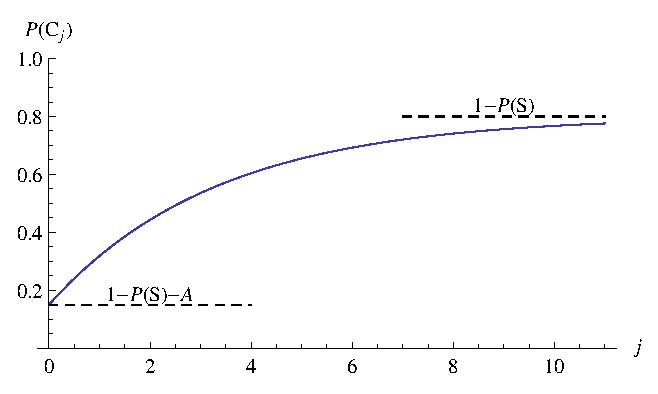
\includegraphics{exponential.eps}
\caption{The Bayesian Knowledge Tracing model in functional form. 
          $P_j(C)$ the probability of  the student getting step $j$ correct.}
 \label{bktgraph}
\end{figure}

This model can be  solved exactly.  First, we rewrite (\ref{recurse}) in a
more suggestive form:
%
\begin{equation}
        1-P_j = \left(1-P(L)\right) \left(1-P_{j-1}\right) \; .
\end{equation}
%
One can show that this recursion relation has solutions of the form:
%
\begin{equation}
            1-P_j = \left(1-P(L)\right)^j\left(1-P_0\right) \; .
	    \label{sol}
\end{equation}
%
%
Substituting (\ref{sol}) into (\ref{pnc}), we get:
%
\begin{equation}
         P_j(C) = 1-P(S) -\left(1-P(S)-P(G)\right) \left(1-P_0\right)
                   \left(1-P(L)\right)^j \; . \label{pncsoln}
\end{equation}
%
Note that the form of $P_j(C)$, as a function of $j$, 
depends on only {\em three} parameters:  $P(S)$, $P(L)$, and 
$\left(1-P(S)-P(G)\right) \left(1-P_0\right)$.
If we define
%
\begin{equation} 
          A=\left(1-P(S)-P(G)\right) \left(1-P_0\right)  \label{aa}
\end{equation}
%
 and $\beta=-\log(1-P(L))$, then we can rewrite (\ref{pncsoln}) in 
a clearer form:
%
\begin{equation}
         P_j(C) = 1-P(S) -A e^{-\beta j} \, .
\end{equation}
%
Thus, $P_j(C)$ is an exponential; see Fig.~\ref{bktgraph}.

\section{Identifiability and Model Degeneracy}


\begin{figure}
\centering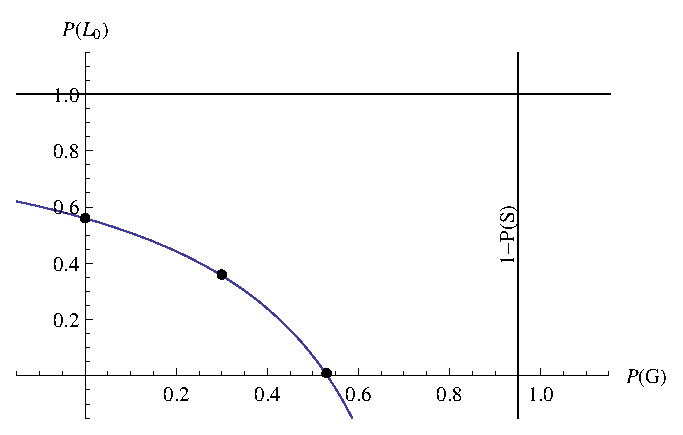
\includegraphics{table1.eps}
\caption{Relation between $P(G)$ and $P_0$ for the BKT model
  described in Table~1 of \cite{beck_identifiability:_2007}.  
  The line is from Eqn.~(\ref{aa}), with $P(S)=0.05$ and $A=0.418$.
  The three points are the  three parameter sets listed in Table~1 of
  \cite{beck_identifiability:_2007}. 
 }
 \label{table1}
\end{figure}


The fact that the BKT model is a function of three parameters
was first noticed by Beck and Chang~\cite{beck_identifiability:_2007} 
where they call it the ``Identifiability Problem.''   In their paper, 
they noted that multiple
combinations of $P(G)$ and $P_0$ give exactly the same $P_j(C)$, but
failed to explain why this is the case.  An example showing the relation
between $P(G)$ and $P_0$ for a given model is shown in Fig.~\ref{table1}.
Thus, we can see that Eqn.~(\ref{aa}) provides an explanation of the
Identifiability Problem.

Baker, Corbett, and Aleven~\cite{baker_more_2008} discuss the need for 
model parameters to be physically meaningful.  They call this 
``Model Degeneracy.''   For example, all probabilities should lie between zero and one.  
In the case of the BKT model, we demand that $0\le P_0\le 1$ and
 $0\le P(G) \le 1$.
If we further demand that learning is positive (which may or may not be justified
by empirical data), then we have the constraint $A>0$ or $P(G)<1-P(S)$.
These constraints on $P_0$ and $P(G)$ correspond to the rectangular region shown in Fig.~\ref{table1}.
In terms of $A$, valid values of $P(G)$ and $P_0$ occur when
$0<A<1-P(S)$; for negative learning, valid values occur when
$-P(S)<A<0$.  This sets the range of physically meaningful values of
$A$ when fitting to student data.

\section{Bayesian Knowledge Tracing Algorithm}

\begin{figure}
\centering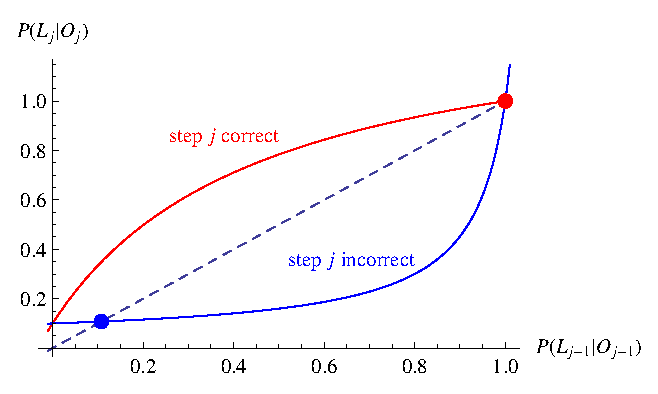
\includegraphics{p-recursion.eps}
\caption{
  Recursion relations the BKT model, Eqns.~(\ref{correct}) and 
  (\ref{incorrect}).
  The stable fixed point for each recursion relation is marked
  by a dot.  Since the ``step $j$ correct'' curve is above the
  dashed line, Eqn.~(\ref{correct}) causes $P_j$ to 
   converge to the fixed point at 1.  Likewise, since 
   the ``step $j$ incorrect'' curve is below the line, 
   Eqn.~(\ref{incorrect}) causes $P_j$ to converge 
   to the lower fixed point~(\ref{incorrectfixedpoint}).
 }
 \label{p-recursion}
\end{figure}


So far, we have discussed using BKT as a model which, when expressed
in functional form, can be fitted to empirical data to obtain values
for the three model parameters.  In order to predict $P_j$ for an
individual student in real time, an alternative form is often used where
$P_j$ is updated using the data from the student itself.
In this case, the recursion relation for updating $P_j$ 
\cite{corbett_knowledge_1994,baker_more_2008} depends on
student performance on that step:
%
\begin{eqnarray}
       P_j &=&
       1-\frac{\left(1-P(L)\right)\left(1-P_{j-1}\right)P(G)}{P(G)+\left(1-P(S)-P(G)\right)
         P_{j-1}}  \mbox{~,~~ step $j$ correct} \label{correct}\\
       P_j &=& 1-\frac{\left(1-P(L)\right)\left(1-P_{j-1}\right)\left(1-P(G)\right)}
                                 {1-P(G)-\left(1-P(S)-P(G)\right) P_{j-1}}
                        \mbox{~ ,~~ step $j$ incorrect.} \label{incorrect}
\end{eqnarray}
%
While these recursion relations cannot be solved analytically, we
can learn much about their solutions by conducting a fixed point analysis.
First, we find the fixed points of each recursion, (\ref{correct}) and
(\ref{incorrect}), by setting $P_j=P_{j-1}$.  For Eqn.~(\ref{correct}), we
find a stable fixed point at $1$ and an unstable fixed point at
\begin{equation}
    - \frac{P(G) P(L)}{1-P(G)-P(S)} \; .
      \label{correctfixedpoint}
\end{equation}
Similarly, Eqn.~(\ref{incorrect}) has an unstable fixed point at $1$
and a stable fixed point at
\begin{equation}
    \frac{\left(1-P(G)\right) P(L)}{1-P(G)-P(S)} \; . 
       \label{incorrectfixedpoint}
\end{equation}
The stable fixed points are plotted in Fig.~\ref{p-recursion}.

In order for $P_j$ to remain in the interval $\left[0,1\right]$ 
for any starting value $P_0\in \left[0,1\right]$ and any sequence of 
correct/incorrect steps, 
we need the stable fixed point (\ref{incorrectfixedpoint})
to lie in the interval $\left[0,1\right]$ and the unstable fixed point 
(\ref{correctfixedpoint}) to remain negative.  This gives us the following
constraints on allowed values for the model parameters:
%
\begin{eqnarray}
        P(G)+P(S)&<& 1 \\
        0 < P(L) &<& 1-\frac{P(S)}{1-P(G)}  \; .
        \label{bigconstraint}
\end{eqnarray}
%
Note that these constraints do not allow for the model to
exhibit negative learning ($A<0$):  such parameter
choices can lead to $P_j$ straying outside the physical
region $\left[0,1\right]$.

The ``Identifiability Problem'' for this model in this form
does not exist, so long as there are both correct and incorrect steps.
This fact can be seen by examining Eqns.~(\ref{correct}) and (\ref{incorrect})
where we see that $P(G)$ has a different functional form in each.
Thus, any rescaling of $1-P_j$ cannot be compensated for by a rescaling
of the parameters in both  (\ref{correct}) and (\ref{incorrect}).

For the ``Model Degeneracy'' issue, we see that (\ref{bigconstraint})
provides a significant constraint on allowed values of model parameters.
It would be interesting to see of often this constraint is 
violated in real tutor systems, such as the 
Cognitive Tutors~\cite{ritter_cognitive_2007}, 
where BKT is applied in this form.


\section{Conclusion}


In conclusion, the Bayesian Knowledge Tracing model, when expressed
in functional form, is an exponential function with three parameters.
It is unclear how the Identifiability Problem has affected previous
results.  Certainly, any study that relies on a value for $P(G)$ or
$P_0$ as output from a fit to student data would be affected.
On the other hand, studies that rely only on $P(S)$ or $P(L)$ from
a fit to student data should be OK.  In addition, expressing
the model in terms of three parameters should improve speed
and accuracy of any maximum likelihood fit to student data.

Some authors have addressed the Identifiability Problem by 
fixing $P_0$ using some arbitrary constraint such as setting
$P_0=0$~\cite{jose_gonzalez-brenes_dynamic_2012}. 
Another popular approach is to use Dirichlet 
priors~\cite{beck_identifiability:_2007} to bias the
parameters towards certain values.  However, one must provide
some additional theoretical justification for the
particular priors chosen.

We see that BKT algorithm does not have
the Identifiability Problem:  all four model parameters
affect model behavior separately.  Thus, it is important to determine
sensible values for all four model parameters.
We also see that, for the model to behave properly,  there are 
significant constraints on allowed values for $P(S)$, $P(G)$, and $P(L)$.

Finally, we see that the functional form of BKT corresponds 
to an exponential, rather than a power law.  
Heathcote, Brown, and Mewhort~\cite{heathcote_power_2000}
argue that learning for individuals is better described by an
exponential while (as shown in earlier studies) learning averaged
over individuals is better described by a power law function.
This suggests that BKT may be more appropriate for describing
individual learners, rather than performance averaged over students.
This contradicts the popular practice of fitting BKT to 
student-averaged data.

\begin{acks}
I would like to thank Ken Koedinger and Tristan Nixon for
useful comments.
\end{acks}

\bibliography{education-modeling}

\end{document}